% Figure 4 of docs/exposition.md: the planted pair drawn on the board of
% Section 2, with I = 1 and zero positions J = (4,1,2,3). The two inputs differ
% only at X_1[4] and in the cell B_{1,10}. Build with tools/render_papers.py.
\documentclass[tikz,border=4pt]{standalone}
% Shared TikZ style for the figures of docs/exposition.md.
% Palette and bit cells follow docs/figures/expert_column.tex.
\usepackage{amsmath,amssymb}
\usetikzlibrary{arrows.meta,positioning,calc,decorations.pathreplacing}
\definecolor{one}{RGB}{226,232,240}
\definecolor{zero}{RGB}{40,40,40}
\definecolor{win}{RGB}{176,58,46}
\definecolor{addr}{RGB}{40,90,150}
\definecolor{lose}{RGB}{110,110,110}
\tikzset{
  bit/.style={draw=black!60, minimum width=4.4mm, minimum height=4.4mm,
              inner sep=0pt, font=\scriptsize},
  onebit/.style={bit, fill=one},
  zerobit/.style={bit, fill=zero, text=white},
  cell/.style={draw=black!50, fill=white, minimum width=10mm,
               minimum height=4.2mm, inner sep=0pt, font=\scriptsize},
  >={Stealth[length=2.2mm]}}

% \boardcolumn{name}{x}{b1}{b2}{b3}{b4}{address text}
% Draws X_name as four bits at height 0 starting at x, the address inputs
% below, and the four cells 00,01,10,11 named <name>c00 ... <name>c11.
\newcommand{\boardcolumn}[7]{%
  \node[anchor=east, font=\small] at (#2-0.05,0) {$X_{#1}$};
  \foreach \c/\b in {1/#3,2/#4,3/#5,4/#6} {
    \ifnum\b=0
      \node[zerobit] (x#1-\c) at (#2+0.46*\c-0.23,0) {0};
    \else
      \node[onebit] (x#1-\c) at (#2+0.46*\c-0.23,0) {1};
    \fi}
  \node[font=\scriptsize, align=center, addr, anchor=north] (adr#1)
    at (#2+0.92,-0.38) {#7};
  \foreach \s/\k in {00/0,01/1,10/2,11/3} {
    \node[cell] (#1c\s) at (#2+0.92,-1.62-0.5*\k) {$B_{#1,\s}$};}
}

\begin{document}
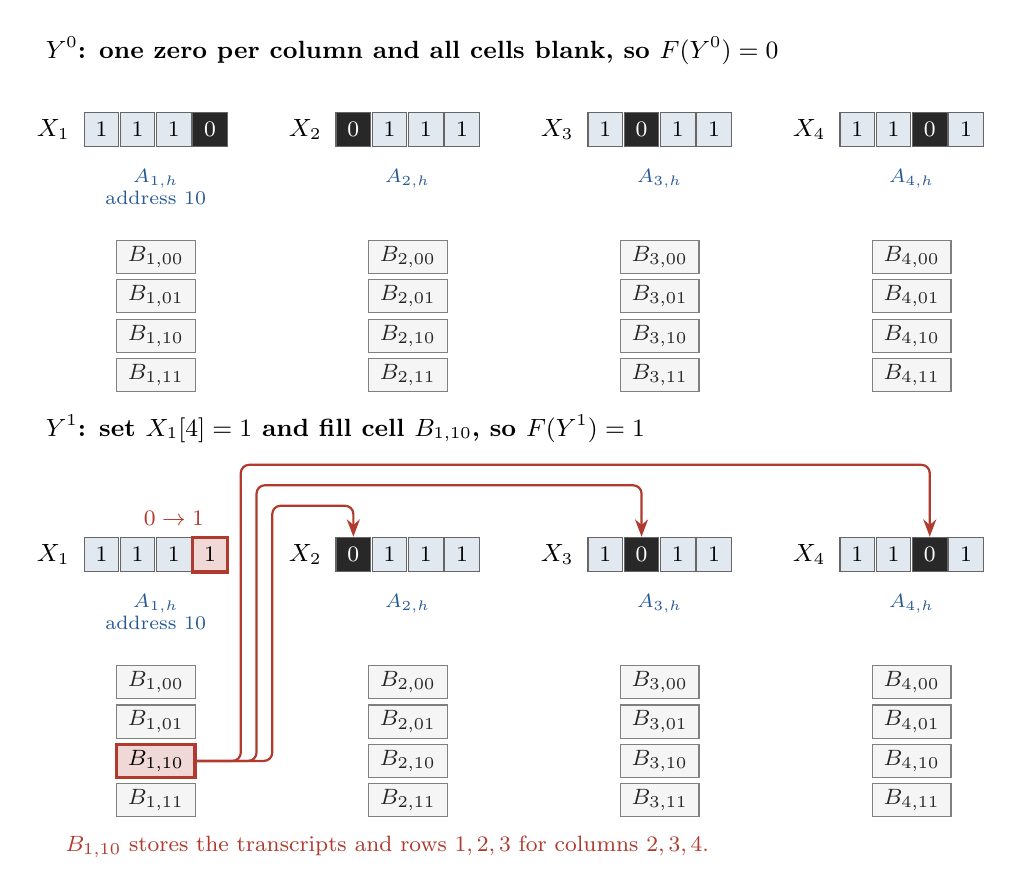
\begin{tikzpicture}
\tikzset{cell/.append style={fill=black!4, text=black!85, font=\footnotesize},
        bit/.append style={font=\footnotesize}}
% ---- dummy input Y^0 ---------------------------------------------------
\begin{scope}
\node[font=\small\bfseries, anchor=west] at (-0.6,1.0)
  {$Y^0$: one zero per column and all cells blank, so $F(Y^0)=0$};
\boardcolumn{1}{0}{1}{1}{1}{0}{$A_{1,h}$\\address $10$}
\boardcolumn{2}{3.2}{0}{1}{1}{1}{$A_{2,h}$}
\boardcolumn{3}{6.4}{1}{0}{1}{1}{$A_{3,h}$}
\boardcolumn{4}{9.6}{1}{1}{0}{1}{$A_{4,h}$}
\end{scope}
% ---- planted input Y^1 -------------------------------------------------
\begin{scope}[shift={(0,-5.4)}]
\node[font=\small\bfseries, anchor=west] at (-0.6,1.6)
  {$Y^1$: set $X_1[4]=1$ and fill cell $B_{1,10}$, so $F(Y^1)=1$};
\boardcolumn{1}{0}{1}{1}{1}{1}{$A_{1,h}$\\address $10$}
\boardcolumn{2}{3.2}{0}{1}{1}{1}{$A_{2,h}$}
\boardcolumn{3}{6.4}{1}{0}{1}{1}{$A_{3,h}$}
\boardcolumn{4}{9.6}{1}{1}{0}{1}{$A_{4,h}$}
\node[onebit, draw=win, very thick, fill=win!20] at (x1-4) {1};
\node[cell, fill=win!20, draw=win, very thick, text=black] at (1c10) {$B_{1,10}$};
\draw[->, win, thick, rounded corners=3pt]
  (1c10.east) -- (2.4,-2.62) -- (2.4,0.62) -| (x2-1.north);
\draw[->, win, thick, rounded corners=3pt]
  (1c10.east) -- (2.2,-2.62) -- (2.2,0.88) -| (x3-2.north);
\draw[->, win, thick, rounded corners=3pt]
  (1c10.east) -- (2.0,-2.62) -- (2.0,1.14) -| (x4-3.north);
\node[win, font=\footnotesize, align=left, anchor=north west] at (-0.35,-3.45)
  {$B_{1,10}$ stores the transcripts and rows $1,2,3$ for columns $2,3,4$.};
\node[win, font=\footnotesize, anchor=south] at (1.15,0.25) {$0\to1$};
\end{scope}
\end{tikzpicture}
\end{document}
